\section{Deep Reinforcement Learning}
\label{sec:drl}


\subsection{Deep Neural Networks}

\subsubsection{History of NNs}

\begin{itemize}
    \item[\textbf{1940}]: Electronic brain
    \item[\textbf{1957}]: The perceptron 
    \item[\textbf{1960-1970}]: Golden Age, ADALINE: first single layer neural network. 
    \item[\textbf{1970-1986}]: The XOR problem spawns the Dark Age (AI Winter). 
    \item[\textbf{1986}]: Multi-layered perceptron + backpropagation 
    \item[\textbf{1995}]: Support Vecor Machines 
    \item[\textbf{2006}]: Deep Neural Networks
\end{itemize}

\subsubsection{Notes}

\begin{itemize}
    \item Changing parameters according to the error measurement will cause the system to jump around to much and be very effected by noise. That is why the learning rate is introduced.
    \item Observations suggest neurons do not react readily, but instead suppress the input until it has grown large enough to trigger the output. This notion of a threshold is implemented by the activation function.
\end{itemize}


\subsection{The large state space problem}

Both value iteration and Q-learning does a loop over all states. This is challenging when the state space is very large. E. g. the Atari game has $128*{33600}$ possible frame configurations -> billions of billions of years to enumerate all possible states -> curse of dimensionality, recognized by Bellman.

Instead, we want to use a nonlinear representation that maps both state and action onto a value, as a regression problem. This is a job for neural networks.

\subsubsection{Deep Q-learning (DQN)}

The model in DQN is a convolutional neural netwok, trained with a variant of Q-learning, whose input is raw pixels and whose output is a value function estimating future rewards. \textbf{The network estimates the action-value function Q}.

The estimation of Q(s, a) by parameter vector $\theta$ is given as $Q(s', a'; \theta)$. 

\begin{align}
    Q(s, a) &\longleftarrow Q(s, a) + \alpha(r + \gamma \max_a' Q(s', a') - Q(s, a)) \\
    \theta  &\longleftarrow \theta + \alpha(r + \gamma \max_a' Q(s', a'; \theta) - Q(s, a; \theta))\nabla_{\theta}Q(s', a'; \theta)
\end{align}

\subsection{The challenges of Deep Reinforcement Learning}

\begin{itemize}
    \item In RL, both the input and the target change constantly during the training process, which makes training unstable. Hard to learn a mapping that is constantly changing.
    \item In supervised learning, the label stays the same for a given input, and this makes every batch have the same data distribution. Samples are also independent of each other in the same batch. 
    \item Thus, a problem for RL algorithms is that the data is \textbf{highly correlated} and there are \textbf{non-stationary probability distributions}.
\end{itemize}

\textbf{Solutions to challenges}

\begin{itemize}
    \item Experience replay: Randomly sampling previous transitions and replay this. This smoothens the training distribution over many past behaviours.
    \item Make the system obtain a separate target network with weight-vector $\theta^-$ to create a temporal gap between the target action-value function and the action-value function that updates continually.
\end{itemize}

\begin{figure}[h]
    \centering
        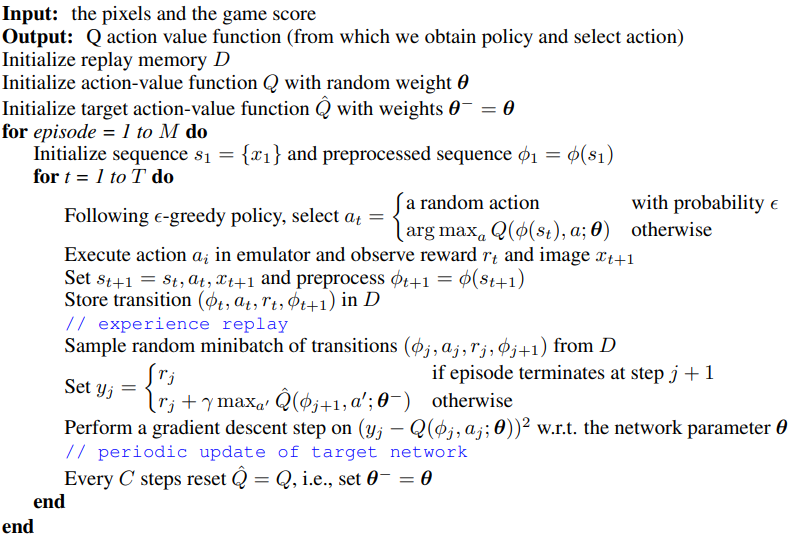
\includegraphics[width=\textwidth]{figures/DRL/dqn.PNG}\\
        \caption{Deep Q-learning pseudocode.}
\end{figure}

The gradient descent step is performed based on the least squares measure of the difference of the reward we obtained and the discounted target action-value function from that step, and the action-value function defined by the network parameter $\theta$.